\documentclass[10pt,landscape]{article}
\usepackage[italian]{babel}
\usepackage[utf8]{inputenc}
\usepackage{multicol}
\usepackage{calc}
\usepackage{ifthen}
\usepackage[landscape]{geometry}
\usepackage{hyperref}
\usepackage{amsmath}
\usepackage{amssymb}
\usepackage{tabularx}
\usepackage{caption}
\usepackage{verbatim}
\usepackage{systeme}
\usepackage{nicefrac}
\usepackage{accents}
\usepackage{enumitem}
\usepackage[printwatermark]{xwatermark}
\usepackage{tikz}
\usetikzlibrary{calc,matrix}
\usepackage[compact]{titlesec}
\usepackage{microtype}
\usepackage[flushleft]{threeparttable}
\usepackage{textcomp}
\usepackage{pifont}
\usepackage{pgfplots}
\usepackage{float}
\usepackage{mathtools}
\usepackage{todonotes}
\usepackage[ruled,vlined]{algorithm2e}

% This sets page margins to .5 inch if using letter paper, and to 1cm
% if using A4 paper. (This probably isn't strictly necessary.)
% If using another size paper, use default 1cm margins.
\ifthenelse{\lengthtest { \paperwidth = 11in}}
{ \geometry{top=.5in,left=.5in,right=.5in,bottom=.5in} }
{\ifthenelse{ \lengthtest{ \paperwidth = 297mm}}
	{\geometry{top=1cm,left=1cm,right=1cm,bottom=1cm} }
	{\geometry{top=1cm,left=1cm,right=1cm,bottom=1cm} }
}

% Turn off header and footer
\pagestyle{empty}

% Reduce size of \section e \subsection
\titleformat{\section}{\normalfont\large\bfseries}{\thesection}{1em}{}
\titleformat{\subsection}{\normalfont\normalsize\bfseries}{\thesubsection}{1em}{}
\titlespacing{\section}{0pt}{0ex}{-0.5ex}
\titlespacing{\subsection}{0pt}{0ex}{-0.5ex}

% Define BibTeX command
\def\BibTeX{{\rm B\kern-.05em{\sc i\kern-.025em b}\kern-.08em
		T\kern-.1667em\lower.7ex\hbox{E}\kern-.125emX}}

% Don't print section numbers
\setcounter{secnumdepth}{0}


\setlength{\parindent}{0pt}
\setlength{\parskip}{0pt plus 0.5ex}

\setlist[itemize]{noitemsep, nolistsep}

% No algorithm numbering
\renewcommand{\thealgocf}{}
% do-while
\SetKwRepeat{Do}{do}{while}

\newcommand{\rarr}{\rightarrow}

\newcommand{\cmark}{\ding{51}}%
\newcommand{\xmark}{\ding{55}}%


\newwatermark[allpages,color=black!10,angle=45,scale=6,xpos=-20,ypos=15]{DRAFT}

\begin{document}

\raggedright
\footnotesize
\begin{multicols}{3}

% multicol parameters
% These lengths are set only within the two main columns
%\setlength{\columnseprule}{0.25pt}
\setlength{\premulticols}{1pt}
\setlength{\postmulticols}{1pt}
\setlength{\multicolsep}{1pt}
\setlength{\columnsep}{2pt}

{\Large{\textbf{Formal Languages and Compilers}}}

\section{Closure Properties}

Let $L \in CF$, $D \in DET$, and $R \in REG$

\begin{table}[H]
    \centering
    \begin{tabularx}{\textwidth}{| r | r | r |}
        $R^R \in REG$ & $L^R \in CF$ & $D^R \notin DET$ \\
        $R^* \in REG$ & $L^* \in CF$ & $D^* \notin DET$ \\
        $\neg R \in REG$ & $\neg L \notin CF$ & $\neg D \in DET$ \\
        $R \cup R \in REG$ & $L \cup L \in CF$ & $D_1 \cup D_2 \notin DET$ \\
        & & $D \cup R \in DET$ \\
        $R . R \in REG$ & $L . L \in CF$ & $D_1.D_2 \notin DET$ \\
        & & $D.R \in DET$ \\
        $R \cap R \in REG$ & $L \cap L \notin CF$ & $D \cap D \notin DET$ \\
        & $L \cap R \in CF$ & $D \cap R \in DET$ \\
    \end{tabularx}
\end{table}

\section{Types of Rules}

\begin{table}[H]
    \centering
    \begin{tabularx}{\textwidth}{| l | c |}
        Terminal & $\rarr a | \epsilon$ \\
        Empty & $\rarr \epsilon$ \\
        Initial & $S \rarr$ \\
        Recursive & $A \rarr \alpha A \beta$ \\
        Left-Recursive & $A \rarr A \beta$ \\
        Right-Recursive & $A \rarr \alpha A$ \\
        Left-Right-Recursive & $A \rarr A \alpha A$ \\
        Copy/Categorization & $A \rarr B$ \\
        Linear & $\rarr u A v | w$ \\
        Left-Linear & $\rarr A v | w$ \\
        Right-Linear & $\rarr v A | w$ \\
        Homogeneous Normal & $\rarr A_1\ldots A_n | a$ \\
        Chomsky Normal & $\rarr AB | a$ \\
        Greibach Normal & $\rarr a\sigma | b$ \\
        Operator Normal & $\rarr A a B$ \\
    \end{tabularx}
\end{table}

\section{Reachable nonterminals}

$A$ is reachable iif $S \Rightarrow^* \alpha A \beta$

For finding the reachable nonterminals build the \textbf{produce} graph and visit it from the axiom.

\section{Defined nonterminals}
$A$ is defined iff $L_A(G) \ne \emptyset$.

For finding the defined nonterminals apply the following relations:
\begin{align*}
    D &:= \{ A | (A \rarr u) \in P, u \in \Sigma^*\} \\
    D &:= D \cup \{ A | (A \rarr B_1\ldots B_n) \in P, \land \forall B_i: B_i \in (D \cup \Sigma) \}
\end{align*}

\section{Circular Derivations}

Derivations like $A \Rightarrow^+ A$, are not essential and introduce ambiguity.

\section{Clean Grammars}
A grammar $G$ is clean iif every nonterminal is \textbf{reachable} and every nonterminal is \textbf{defined}.

\section{Useful Languages}

\paragraph{Dyck Language} $S \rarr bSeS | \epsilon$
\paragraph{Math Expressions}
\begin{align*}
    E &\rarr E + T | T \\
    T &\rarr T * F | F \\
    F &\rarr (E) | i
\end{align*}

\section{Ambiguity}

A sentence $x$ of $G$ is ambiguous iff it admits different syntax trees. In that case $G$ is ambiguous. The degree of ambiguity of $x$ is the number of distinct trees of $x$, of $G$ is the maximum over its sentences.

\paragraph{Bilateral Recursions} $E \rarr E + E | i$ becomes $E \rarr i + E | i$.

\paragraph{Left-Right Recurions in different rules} $A \rarr aA | Ab | c$. Remedies: generate using different rules or force an order of derivation.

\paragraph{Union of Languages} If $L_1 \cap L_2 \ne \emptyset$ then $L_1 \cup L_2$ is ambiguous (the intersection has 2 derivations). Remedy: provide disjointed set of rules: $L_1 \cap L_2$, $L_1 \setminus L_2$ and $L_2 \setminus L_1$.

\paragraph{Concatenation of Languages} $G_1 . G_2$ is ambiguous if $\exists x_1 \in L_1, x_2 \in L_2$ such that $x_1 = uv$ with $u \in L_1$ and $x_2 = vz$ with $z \in L_2$: $uvz$ can be $(uv)z$ or $u(vz)$.

\paragraph{Inherent Ambiguity} A language is inherently ambiguous if all its grammar are ambiguous, e.g. those where the intersection is not CF.

\paragraph{Lack of Order in Derivations} $S \rarr bSc | bbSc | \epsilon$ becomes $S \rarr bSc | D$, $D \rarr bbDc | \epsilon$.

\section{Grammar Equivalence}

\paragraph{Weak Equivalence} $G_1$ weakly equivalent to $G_2$ iff $L(G_1) = L(G_2)$ (even with different trees). It is not decidable.

\paragraph{Strong Equivalence} If weak equivalent and same condensed skeleton trees.

Strong $\Rightarrow$ Weak

\section{Grammar Transformations}

\subsection{Expansion of a nonterminal}
Eliminate a nonterminal: $A \rarr \alpha B \gamma$, $B \rarr \beta_1 | \ldots | \beta_n$ becomes $A \rarr \alpha \beta_1 \gamma | \ldots | \alpha \beta_n \gamma$.

It's always possible to remove the axiom from the right part by adding a new axiom $S_0 \rarr S$.

\subsection{Elimination of empty rules}
A nonterminal is \textbf{nullable} iff it exists a derivation $A \Rightarrow^+ \epsilon$.
\begin{align*}
    A \in \text{Null} &\text{ if }A \rarr \epsilon \in P \\
    A \in \text{Null} &\text{ if } A \rarr A_1\ldots A_n \in P, A_i \in V \setminus \{A\} \land \forall A_i (A_i \in \text{Null})
\end{align*}
\textbf{Note}: Recursive rules cannot be used.

\paragraph{Construction of the non-nullable normal form}
\begin{itemize}
    \item Compute the Null set.
    \item For each rule add as alternative all the combinations of removing the nullable nonterminals.
    \item Remove all empty rules ($A \rarr \epsilon$) excpet for $A = S$.
    \item Clean the grammar and remove circularity.
\end{itemize}

\textbf{Example} $S \rarr SAB | AC$, $A \rarr aA | \epsilon$, $B \rarr bB | \epsilon$, $C \rarr cC | c$. Null is $\{A, B\}$, remove $A$ and $B$ from the rules in every combination: $S \rarr SAB | SA | SB | S | AC | C$, $A \rarr aA | a$, $B \rarr bB | b$, $C \rarr cC | c$. Then remove circularity ($S \rarr S$).

\subsection{Elimination of copy rules}
$\text{Copy}(A) = \{ B \in V | A \Rightarrow^* B \}$.

Assuming \textbf{grammar with no empty rules}, apply until a fixed point:
\begin{align*}
    A &\in \text{Copy}(A) \\
    C &\in \text{Copy}(A) \text{ if } B \in \text{Copy}(A) \land B \rarr C \in P
\end{align*}

\paragraph{Construction of the grammar without copy rules}

\begin{itemize}
    \item Remove copy rules: $P' := P \setminus \{A\rarr B | A, B \in P\}$
    \item Add compensating rules: $P' := P' \cup \{ A \rarr \alpha | \exists B (B \in \text{Copy}(A) \land (B \rarr \alpha \in P)) \}$
\end{itemize}

\textbf{Example} $E \rarr E + T | T$, $T \rarr T \times C | C$, $C \rarr 0|\ldots|9$.
$\text{Copy}(E)=\{E,T,C\}$, $\text{Copy}(T) = \{T, C\}$, $\text{Copy}(C) = \{C\}$.
The grammar becomes $E \rarr E+T|T\times C|0|\ldots|9$, $T \rarr T\times C|0|\ldots|9$, $C \rarr 0|\ldots|9$.

\subsection{Conversion from left to right recursion}

\paragraph{Immediate L-recursions} $A \rarr A\beta_1 | \ldots | A\beta_h$ where no $\beta_i$ is empty, $A \rarr \gamma_1 | \ldots | \gamma_k$. Introduce new nonterminal $A'$:
\begin{align*}
    A &\rarr \gamma_1A' | \ldots | \gamma_kA' | \gamma_1 | \ldots | \gamma_k \\
    A' &\rarr \beta_1A' | \ldots | \beta_hA' | \beta_1 | \ldots | \beta_h
\end{align*}

\textbf{Example} $E \rarr E+T | T$, $T \rarr T\times F | F$, $F \rarr (E) | i$. It becomes $E \rarr TE' | T$, $E' \rarr +TE'|+T$, $T \rarr FT'|F$, $T' \rarr \times FT'|\times F$, $F\rarr (E)i$.

\textbf{Non-Immediate L-recurions} are much harder and not covered by the slides.

\section{Unilinear Grammar}

A grammar is unilinear iff all rules are either all left-linear or right-linear. It can also be required that it has:
\begin{itemize}
    \item Strictly unilinear rules: $A \rarr aB$ with $a\in \Sigma \cup \epsilon$ and $B \in V \cup \epsilon$
    \item All terminal rules are empty: $B \rarr b$ replaced with $B \rarr bB'$, $B' \rarr \epsilon$
\end{itemize}

\subsection{From Unilinear to Regular Expression}

\textbf{Assumptions}: strictly right unilinear, all terminal rules empty.

For every nonterminal $A$ defined by $A \rarr a_1A_1|\ldots|a_kA_k|\epsilon$:
$L_A = a_1L_{A_1} \cup | \ldots | \cup a_kL_{A_k} \cup \epsilon$

\textbf{Arden Identity}: $X = KX \cup L$ (with $K$ nonempty) has exactly one solution $X = K^*L$.

\textbf{Example} $S \rarr sS | eA$, $A \rarr sS|\epsilon$
\begin{alignat*}{2}
&
    \begin{cases}
        L_S = sL_S \cup eL_A \\
        L_A = sL_S \cup \epsilon
    \end{cases}
&&
    \begin{cases}
        L_S = sL_S \cup e(sL_S \cup \epsilon) \\
        L_A = sL_S \cup \epsilon
    \end{cases}
\\
&
    \begin{cases}
        L_S = (s \cup es) L_S \cup e \\
        L_A = sL_S \cup \epsilon
    \end{cases}
&&
    \begin{cases}
        L_S = (s \cup es)^*e \\
        L_A = sL_S \cup \epsilon = s(s \cup es)^*e \cup \epsilon
    \end{cases}
\end{alignat*}


\section{Clean Automata}

A state is $q$ \textbf{reachable} from $p$ if there is a computation from $p$ to $q$.
A state is \textbf{accessible} if it is reachable from the initial state.
A state is \textbf{post-accessible} if a final state can be reached from it.
A state is \textbf{useful} if it is accessible and post-accessible.

An automaton is \textbf{clean} if all the states are useful.

\section{Minimal Automaton}

\textbf{Assumption}: the automaton is clean except for the $q_{err}$ state.

State $p$ is indistinguishable from $q$ iff $\forall x, \delta(p,x)$ and $\delta(q, x)$ are both final or non-final. Indistiguishability is an equivalence relation, 2 indistinguishable states can be merged with no change in the language recognized.

\subsection{Compute distinguishability set}
$p$ is distinguishable from $q$ iff
\begin{itemize}
    \item $p$ is final and $q$ is not, or vice-versa; or
    \item $\exists a: \delta(p, a)$ is distinguishable from $\delta(q, a)$
\end{itemize}

\textbf{Example}
\begin{figure}[H]
    \centering
    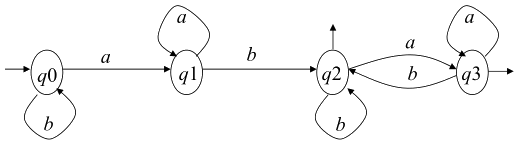
\includegraphics[width=\linewidth]{automata/example-automaton-minimization.png}
\end{figure}

\begin{table}[H]
    \centering
    \begin{minipage}{0.35\linewidth}
        \begin{tabular}{r|c|cc}
            \cline{2-2}
            $q_1$ & & & \\
            \cline{2-3}
            $q_2$ & \xmark & \multicolumn{1}{c|}{\xmark} & \\
            \cline{2-4}
            $q_3$ & \xmark & \multicolumn{1}{c|}{\xmark} & \multicolumn{1}{c|}{} \\
            \cline{2-4}
            \multicolumn{1}{c}{} & \multicolumn{1}{c}{$q_0$} & $q_1$ & $q_2$
        \end{tabular}
    \end{minipage}
    \begin{minipage}{0.6\linewidth}
        \begin{tabular}{r|c|cc}
            \cline{2-2}
            $q_1$ & (1,1)(0,2) & & \\
            \cline{2-3}
            $q_2$ & \xmark & \multicolumn{1}{c|}{\xmark} & \\
            \cline{2-4}
            $q_3$ & \xmark & \multicolumn{1}{c|}{\xmark} & \multicolumn{1}{c|}{(3,3)(2,2)} \\
            \cline{2-4}
            \multicolumn{1}{c}{} & \multicolumn{1}{c}{$q_0$} & $q_1$ & $q_2$
        \end{tabular}
    \end{minipage}
    \begin{minipage}{0.6\linewidth}
        \begin{tabular}{r|c|cc}
            \cline{2-2}
            $q_1$ & \xmark & & \\
            \cline{2-3}
            $q_2$ & \xmark & \multicolumn{1}{c|}{\xmark} & \\
            \cline{2-4}
            $q_3$ & \xmark & \multicolumn{1}{c|}{\xmark} & \multicolumn{1}{c|}{(3,3)(2,2)} \\
            \cline{2-4}
            \multicolumn{1}{c}{} & \multicolumn{1}{c}{$q_0$} & $q_1$ & $q_2$
        \end{tabular}
    \end{minipage}
\end{table}

States $q_2$ and $q_3$ are indistinguishable, so they can be merged.

\begin{figure}[H]
    \centering
    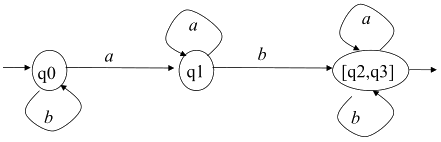
\includegraphics[width=\linewidth]{automata/example-automaton-minimization-2.png}
\end{figure}

\section{Operations on FSA}

\subsection{Reflection}
Given a \textbf{deterministic} FSA.
\begin{itemize}
    \item Switch initial and final states
    \item Reverse the arrow directions
\end{itemize}

\subsection{Complement}
Given a \textbf{deterministic} FSA.
\begin{itemize}
    \item Extend the FSA with the error state: $Q' = Q \cup \{p\}$
    \item Make $\delta$ complete (using $p$)
    \item Switch initial and final states
\end{itemize}

\subsection{Intersection}
$M_1 \cap M_2 = M_3$ where the states of $M_3$ are the cartesian product of the original 2 sets (i.e. all the pairs).
\[
    <q_1, q_2> \xrightarrow{a} <r_1,r_2> \iff q_1\xrightarrow{a} r_1 \land q_2 \xrightarrow{a} r_2
\]

The final/initial states are the ones final/initial for both.

\section{Grammar $\rarr$ Automaton}

Given a \textbf{Right-Linear Grammar}, the automaton has as states the \emph{nonterminals}, the initial state is the axiom.
\begin{align*}
    A \rarr aB &\quad\Rightarrow\quad A \xrightarrow{a} B \\
    A \rarr B & \quad\Rightarrow\quad A \xrightarrow{\epsilon}B \\
    A \rarr \epsilon &\quad\Rightarrow\quad A \rarr \text{ (final)}
\end{align*}

Given a \textbf{Left-Linear Grammar}

LL $\xrightarrow[\text{grammar}]{\text{reverse}}$ RL $\xrightarrow[\text{autom}]{\text{make}}$ automaton $\xrightarrow[\text{automaton}]{\text{reverse}}$ result.

\section{Automaton $\rarr$ Regular Expression}
\textbf{BMC} (Brzozowski \& McCluskey) method.

\textbf{Assumptions}: unique initial state $i$ without incoming arcs, unique final state $t$ without outgoing arcs.

Remove internal states (i.e. not $i$ nor $t$) compensating with new moves.

\begin{figure}[H]
    \centering
    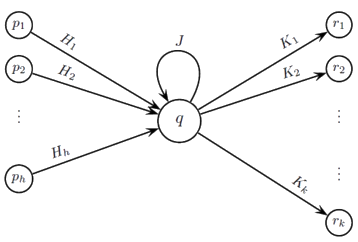
\includegraphics[width=0.5\linewidth]{automata/bmc.png}
\end{figure}

Replace $q$ with: for each pair $p_i$, $r_j$ a compensating transition $p_i \xrightarrow{H_iJ^*K_j} r_j$. All the parallel transitions should be merged ASAP in $p \xrightarrow{e_1|e_2} r$.

\section{Elimination of nondeterminism}

\subsection{Elimination of $\epsilon$-moves}
For each $p \xrightarrow{\epsilon} q$:
\begin{itemize}
    \item For each $q \xrightarrow{a} r$ where $a$ can be anything (including $\epsilon$) add an arc $p \xrightarrow{a} r$
    \item If $q$ was final, $p$ becomes final
    \item Remove $p \xrightarrow{\epsilon} q$
\end{itemize}

\subsection{Berry-Sethi Method}
\begin{itemize}
    \item Number non-$\epsilon$ arcs and add $\dashv$ on exiting final states
    \item Compute $Ini$ and $Fin$ with the same rules as r.e.
    \item Apply Berry-Sethi construction
\end{itemize}
The automaton obtained is deterministic but can be non-minimal.

\section{Regular Expression $\rarr$ Automaton}

\subsection{Thompson method}
Result nondeterministic with $\epsilon$-moves. Map every portion of the r.e. to a piece of the automaton. Every piece of the automaton must have a unique and final state.

\begin{figure}[H]
    \centering
    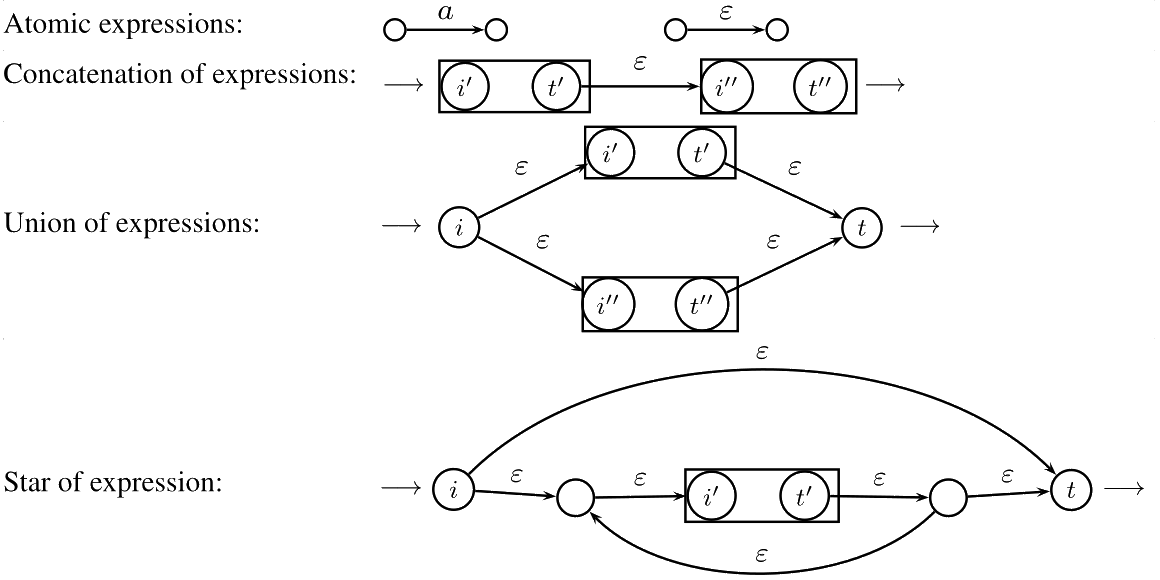
\includegraphics[width=\linewidth]{automata/thompson.png}
\end{figure}

\subsection{Berry-Sethy method}

Result deterministic but can be non-minimal.

\subsubsection{Locally Testable Languages (LOC)}

Proper subfamily of REG. Assuming $a,b \in \Sigma$, $x, y \in \Sigma^*$, define $Ini(L) = \{a | ax \in L\}$, $Fin(L) = \{b | xb \in L\}$, $Dig(L) = \{ab | xaby \in L\}$.

\begin{align*}
    L \in \text{LOC} &\iff \\
    L \setminus \{\epsilon\} = \{&x | Ini(x) \in Ini(L) \land \\
    &Dig(x) \subseteq Dig(L) \land \\
    &Fin(x) \in Fin(L) \}
\end{align*}

To prove that a language is not local provide a string $x\notin L$ s.t. $Ini(x) \in Ini(L) \land Dig(x) \subseteq Dig(L) \land Fin(x) \in Fin(L)$.

\subsubsection{Recognizer for Local Languages}

A unique initial state $q_0$, a state for each terminal, the finals are the $Fin$. If $\epsilon \in L$ then also $q_0$ is final. $q_0$ is connected to the $Ini$, and the states are connected if the pair is in $Dig$.

\subsubsection{Berry-Sethi method}

Given $e$ the initial r.e., $e'$ is the numbered version over alphabet $\Sigma_N$. Conside expression $e' \dashv$. Define for each symbol $a$ of $e'$ the set $Fol(a) = \{b | ab \in Dig(e'\dashv)\}$.

Every state is a subset of $\Sigma_N \cup \{\dashv\}$, containing all the symbols that may follow in the input. The initial state contains $Ini(e'\dashv)$. The states are generated adding transitions until a fixed point is reached. The final states are the ones containing $\dashv$.

\begin{algorithm*}[H]
    \caption{Berry-Sethi}
    \SetAlgoLined
    $q_0 = Ini(e'\dashv)$;
    $Q = \{q_0\}$;
    $\delta=\emptyset$\;
    \While{$\exists q \in Q$ not visited}{
        mark $q$ as visited\;
        \For{$b \in \Sigma$}{
            $q' = \cup_{\forall b_i \in q} Fol(b_i)$\;
            \If{$q' \notin Q$}{
                mark $q'$ as not visited\;
                $Q = Q \cup \{q'\}$
            }
            $\delta = \delta \cup \{q \xrightarrow{b} q'\}$
        }
    }
\end{algorithm*}


\section{Grammar as Network of FSA}

Given a EBNF grammar where every nonterminal has a unique rule. Any transition labelled with a nonterminal $B$ is a call to the automaton $M_B$.

\begin{description}
    \item[Machine] The FSA of a nonterminal
    \item[Automaton] the PDA that accepts $L(G)$
    \item[Net] the set of all machines
\end{description}

The machine $M_A$ must be \emph{normalized}, initial state $0_A$ must have no entering arcs.

\subsection{Followers of nonterminal}
Given a final state of a machine, the \emph{set of followers} if the set of all the terminal characters that can follow exiting the machine (including $\dashv$). Given a state $q_A$:
\[
    Ini(q_A) = Ini(L(q_A)) = \{ a \in \Sigma | a\Sigma^* \cap L(q_A) \ne \emptyset \}
\]

\textbf{Note}: $Ini$ cannot contain $\epsilon$, it is empty iff $L(q_A)=\{\epsilon\}$.
Terminal $a$ is in $Ini(q_A)$ iff:
\begin{align*}
    & \exists \text{ arc } q_A \xrightarrow{a} r_A \\
    & \exists \text{ arc } q_A \xrightarrow{B} r_A \land a \in Ini(0_B) \\
    & \exists \text{ arc } q_A \xrightarrow{B} r_A \land B \text{ is nullable } \land a \in Ini(r_A)
\end{align*}

\section{Pilot Automaton}

\subsection{Parts of a Pilot Automaton}
\begin{figure}[H]
    \centering
    \begin{tikzpicture}
        \draw (0,0) -- (2,0) -- (2,2) -- (0,2) -- (0,0);
        \draw (0,1.33) -- (2,1.33);
        \draw (0.1,1.66) node[anchor=west] {$1_S\qquad \dashv$};
        \draw (0.1,1) node[anchor=west] {$0_A\qquad \dashv$};
        \draw (0.1,0.33) node[anchor=west] {$0_B\qquad a\dashv$};

        \draw[dotted] (0.4,1) ellipse (0.4 and 1.1);
        \draw (0.4,0) node[anchor=north] {kernel};
        \draw[dotted] (1.6,1) ellipse (0.4 and 1.1);
        \draw (1.6,2.1) node[anchor=south] {lookaheads};

        \draw [decorate,decoration={brace,amplitude=3},xshift=-4pt,yshift=0pt]
        (0,1.33) -- (0,2) node [black,midway,xshift=-0.6cm]
        {base};
        \draw [decorate,decoration={brace,amplitude=3},xshift=-4pt,yshift=0pt]
        (0,0) -- (0,1.33) node [black,midway,xshift=-0.8cm]
        {closure};
    \end{tikzpicture}
\end{figure}

\subsection{Closure Function}
Let $C$ be a set of candidates:

\begin{algorithm*}[H]
    \caption{Closure Function}
    \SetAlgoLined
    $K = C$\;
    \Do{nothing changes}{
        \begin{alignat*}{2}
            K = K \cup \{ &\langle 0_B,b \rangle | \exists \langle q,a \rangle \in K \land \\
            & \exists\text{ arc } q\xrightarrow{B} r \text{ in } M \land b \in Ini(L(r).a) \}
        \end{alignat*}
    }
    $closure(C) = K$
\end{algorithm*}

In words:
\begin{itemize}
    \item For each candidate add new candidates with $0_B$ as the kernel.
    \item The lookaheads are $Ini(L(r).a)$, i.e. the characters that can follow $r$, including those due to the nullableness of $r$.
\end{itemize}

\subsection{Construction of the automaton}
Construct the m-states $R = \{I_0, I_1, \ldots\}$ and the state-transition function $\theta$.

\begin{algorithm*}[H]
    \caption{Construction of the automaton}
    \SetAlgoLined
    $R' = \{I_0\}$\;
    \Do{$R \ne R'$}{
        $R = R'$\;
        \For{$I\in R$ and $X\in \Sigma \cup V$}{
            $I' = Closure(\theta(I,X))$\;
            \If{$I' \ne \emptyset$}{
                add arc $I \xrightarrow{X} I'$ to $\theta$\;
                \If{$I'\notin R$}{
                    add $I'$ to $R'$\;
                }
            }
        }
    }
\end{algorithm*}

In words:
\begin{itemize}
    \item Start from the initial m-state built from the closure of the initial state of the axiom.
    \item For each m-state add an arc for the exiting transitions to a new m-state considering all the candidates.
    \item Compute and add the closure to the new m-state.
    \item Add the m-state to the automaton \textbf{if not already present}.
\end{itemize}

\textbf{Note}: shift moves do not change the lookaheads, only closures do.

\section{Conflicts}
\subsection{Shift-Reduce conflict}
Given an m-state, there is a S-R conflict if there is an arc with label $a$, as well as a final state with $a$ in the lookahead set.
\begin{figure}[H]
    \centering
    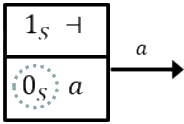
\includegraphics[width=0.2\linewidth]{parsing/shift-reduce-conflict.png}
\end{figure}

\subsection{Reduce-Reduce conflict}
Given an m-state, there are 2 final candidates with a non-empty intersection of the lookahead sets.
\begin{figure}[H]
    \centering
    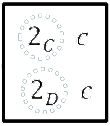
\includegraphics[width=0.15\linewidth]{parsing/reduce-reduce-conflict.png}
\end{figure}

\subsection{Convergent arcs with conflict}
Given 2 candidates in the same m-state, with non-empty intersection lookaheads, which go with a convergent arc to the same state.
\begin{figure}[H]
    \centering
    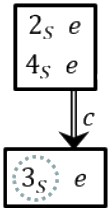
\includegraphics[width=0.15\linewidth]{parsing/convergent-conflict.png}
\end{figure}

\section{ELR Grammars}
After building the pilot automaton check the following:
\begin{itemize}
    \item No shift-reduce conflicts
    \item No reduce-reduce conflicts
    \item No convergence conflicts
\end{itemize}

\todo[inline]{Usage of pilot automaton}

\section{ELL Grammars}

A grammar is ELL iff:
\begin{itemize}
    \item It is ELR
    \item It has the Single Transition Property
    \item It has no Left Recursive Derivations (direct or indirect)
\end{itemize}

\subsection{Single Transition Property}
The STP does not hold if for an m-state there are more transitions possible for a given symbol.

\subsection{Parser Control Flow Graph}

From the machine net:
\begin{itemize}
    \item Add \emph{call arcs}: for $q_A \xrightarrow{B} r_A$ add $q_A \dashrightarrow 0_B$
    \item Add \emph{prospect sets} of the states
    \item Add the \emph{Gui} for the following arcs:
    \begin{itemize}
        \item Terminal shift arc: $q \xrightarrow{a} r$
        \item Call arcs: $q_A \dashrightarrow 0_B$
        \item Exiting arcs of the final states
        \item \textbf{Note}: \textbf{no} \emph{Gui} for nonterminal shift ($q_A \xrightarrow{B} r_A$)
    \end{itemize}
\end{itemize}

\subsection{Prospect sets}
The prospect set of state $q_X$ is the set of symbols that can be encountered when exiting the machine.
It is the union of the lookaheads of all the candidates with $q_X$ as kernel.

\subsection{Guide set}
The guide set ($Gui$) of an arc is the set of symbols that can be met going through that arc.
\begin{itemize}
    \item $Gui(q_A\xrightarrow{a}r_A) = \{a\}$
    \item $Gui(f\rarr) =$ prospect set of $f$ (with $f$ final)
    \item $Gui(q_A\dashrightarrow 0_B) = Ini(L(B)) \cup \{\text{symbols following $B$ if $B$ is nullable}\}$
\end{itemize}

\subsection{Alternative ELL Definition}
A grammar is ELL iff on alternative arcs the guide sets are disjoint.

\subsection{Top-Down Predictive Analyzer}
Based on the PCFG, using a stack initialized with $0_S$. If the top element is $q_A$ (machine $M_A$ is active at the state $q_A$), and the current character is $cc$:
\begin{description}
    \item[Scan] if $q_A \xrightarrow{cc} r_A$: read $cc$, \textbf{pop}, \textbf{push $r_A$}
    \item[Move] if $a_A \dashrightarrow 0_B$ and $q_A \xrightarrow{B} r_A$ and $cc \in Gui(q_A \dashrightarrow 0_B)$: \textbf{pop}, \textbf{push $r_A$}, \textbf{push $0_B$}
    \item[Return] if $q_A$ final, $cc$ in prospect set of $q_A$: \textbf{pop}
    \item[Acceptance] if $A=S$, $q_A$ is final and $cc = \dashv$: \textbf{accept}
\end{description}

\subsection{Increasing lookahead}
If a grammar is not ELL(1) it may be possible that it is ELL(k).
If the guide sets of length $k$ are disjoint the grammar is ELL(k).

\section{Earley Method}

It works on any grammar (even nondeterministic ones) by using a vector of sets.

It builds a vector of size $n+1$ where $n=|x|$ where $E[i]$ is a set of $\langle s,j \rangle$ with $j<i$: $\langle q_A,j \rangle \in E[i]$ means that $x_{j+1\ldots i}$ is derived from $A$ via $0_A\rarr q_A$ in $M_A$.

\begin{algorithm*}[H]
    \caption{TerminalShift(E, i)}
    \SetAlgoLined
    \For{$\langle p,j \rangle \in E[i-1], q\in Q \text{ s.t. } p \xrightarrow{x_i} q$}{
        add pair $\langle q,j \rangle$ to $E[i]$\;
    }
\end{algorithm*}
Add new elements based on terminal shifts, keeping the same \emph{key}.

\begin{algorithm*}[H]
    \caption{Closure(E, i)}
    \SetAlgoLined
    \For{$\langle p,j \rangle \in E[i], X\in V, q\in Q \text{ s.t. } p \xrightarrow{X} q$}{
        add pair $\langle 0_X,i \rangle$ to $E[i]$\;
    }
\end{algorithm*}
Like the closure of Pilot, resetting the \emph{key} to the current index.

\begin{algorithm*}[H]
    \caption{NonTerminalShift(E, i)}
    \SetAlgoLined
    \For{$\langle f,j \rangle \in E[i], X\in V \text{ s.t. } f \text{ is final for } X$}{
        \For{$\langle p,l \rangle \in E[j], q\in Q \text{ s.t. } p \xrightarrow{X} q$}{
            add pair $\langle q,l \rangle$ to $E[i]$\;
        }
    }
\end{algorithm*}
For each final state $\langle q_X,j \rangle$ of the current set, go back to $j$ and search if there is some item that can be advanced using $X$, keep the key found in $j$.

\begin{algorithm*}[H]
    \caption{Completion(E, i)}
    \SetAlgoLined
    \Do{some pair has been added}{
        Closure(E, i)\;
        NonTerminalShift(E, i)\;
    }
\end{algorithm*}

\begin{algorithm*}[H]
    \caption{Earley}
    \SetAlgoLined
    $E[0] = \{\langle 0_S, 0 \rangle \}$\;
    \For{$i = 1$ \KwTo $n$}{
        E[i] = \{\}
    }
    Completion(E, 0)\;
    $i = 1$\;
    \While{$i \le n \land E[i-1] \ne \emptyset$}{
        TerminalShift(E, i)\;
        Completion(E, i)\;
        $i = i + 1$\;
    }
\end{algorithm*}

The input is accepted iff $\langle f_S, 0 \rangle \in E[n]$ (where $f_S$ is final).


\rule{0.3\linewidth}{0.25pt}
\scriptsize\\
\href{mailto:edoardo.morassutto@mail.polimi.it}{Edoardo Morassutto}, Politecnico di Milano, A.A. 2019/2020
\end{multicols}
\end{document}
